\PassOptionsToPackage{dvipsnames}{xcolor}
\documentclass[9pt, xcolor={usenames, dvipsnames}]{beamer}

\usepackage[scale=2]{ccicons}
\usepackage{graphicx}
\usepackage{gensymb}
\usepackage{multimedia}
\usepackage{url}
\usepackage{bookmark}
\usepackage{txfonts}
\usepackage{caption}
\usepackage{subcaption}

% \usepackage{newpxtext,newpxmath}
\usepackage{amsmath,amssymb,amsfonts}

\usepackage{mathpazo}
\usepackage{fontspec}
\setmainfont{TeX Gyre Pagella}

% Backup slides
\usepackage{appendixnumberbeamer}
\usepackage{lipsum}

\setbeamercovered{transparent}

\usepackage[style=authoryear,backend=biber]{biblatex}
\renewcommand*{\nameyeardelim}{\addcomma\addspace}
\addbibresource{bib/abstract.bib}

% Beamer configuration
\usetheme[sectionpage=progressbar, numbering=counter, progressbar=frametitle]{metropolis}

\usepackage{xfp}
\usepackage{pgfplots}
\usepackage{pgfplotsthemetol}
\usepackage{tikz}
\usetikzlibrary{datavisualization.formats.functions, automata, angles, arrows, arrows.meta, backgrounds, calc, decorations.pathreplacing, decorations.markings, decorations.shapes, fit, quotes, shapes.geometric, karnaugh, intersections, patterns, patterns.meta, positioning, shapes, shadings}
\usetikzlibrary{overlay-beamer-styles}
\usepgfplotslibrary{groupplots,units}
\pgfplotsset{width=7cm,compat=1.18}
\usepackage{graphicx}


\tikzset{paint/.style={ draw=#1, fill=#1 },
         decorate with/.style=
{decorate,decoration={shape backgrounds,shape=#1,shape size=1mm,shape sep=.5cm}}}

\makeatletter
\newcommand{\bigcomp}{%
  \DOTSB
  \mathop{\vphantom{\sum}\mathpalette\bigcomp@\relax}
  \slimits@
}
\newcommand{\bigcomp@}[2]{%
  \begingroup\m@th
  \sbox\z@{$#1\sum$}%
  \setlength{\unitlength}{0.9\dimexpr\ht\z@+\dp\z@}%
  \vcenter{\hbox{%
    \begin{picture}(1,1)
    \bigcomp@linethickness{#1}
    \put(0.5,0.5){\circle{1}}
    \end{picture}%
  }}%
  \endgroup
}
\newcommand{\bigcomp@linethickness}[1]{%
  \linethickness{%
      \ifx#1\displaystyle 2\fontdimen8\textfont\else
      \ifx#1\textstyle 1.65\fontdimen8\textfont\else
      \ifx#1\scriptstyle 1.65\fontdimen8\scriptfont\else
      1.65\fontdimen8\scriptscriptfont\fi\fi\fi 3
  }%
}
\makeatother

% Plot style
\pgfplotsset{
    mplot/.style={
        width=.48\textwidth,
        height=.4\textheight,
        grid=major,
        grid style={dashed,gray!30},
        ylabel style={align=center, font=\bfseries\boldmath},
        xlabel style={align=center, font=\bfseries\boldmath},
        x tick label style={font=\bfseries\boldmath},
        y tick label style={font=\bfseries\boldmath},
        scaled ticks=false,
        label style={font=\footnotesize},
        xticklabel style={font=\footnotesize},
        yticklabel style={font=\footnotesize},
        every axis plot/.append style={solid,thick},
    },
}

% Footer
\setbeamertemplate{frame footer}{\underline{Q. Brateau}, Natacha Caouren, F. Le Bars, L. Jaulin, ENSTA Bretagne}

% Block fill
\metroset{block=fill}

% Section pages numbering
\makeatletter
\renewcommand{\metropolis@enablesectionpage}{
  \AtBeginSection{
    \ifbeamer@inframe
      \sectionpage
    \else
      \frame[c,plain]{\sectionpage}
    \fi
  }
}
\metropolis@enablesectionpage
\makeatother

% Title
\title{Modeling and Depth Control of a Subsurface Robot for Low-Cost Marine Robotics Experiments}
\date{September 17, 2025}
\author{\underline{Quentin Brateau}, Natacha Caouren, Fabrice Le Bars, Luc Jaulin}
\institute{ENSTA, 2 rue François Verny, 29200 Brest, France}



\addtobeamertemplate{frametitle}{}{%
    \begin{tikzpicture}[remember picture,overlay]
    \node[anchor=north east,yshift=2pt] at (current page.north east) {
            
\includegraphics[height=0.8cm]{imgs/logo_ensta_bw} 
\includegraphics[height=0.8cm]{imgs/logo_aid_bw}
    };
    \end{tikzpicture}
}


\definecolor{ENSTABlue}{HTML}{3746ff}
\definecolor{ENSTADarkBlue}{HTML}{190f3c}
\definecolor{ENSTACoral}{HTML}{ff808b}

% Progressbar
\setbeamercolor{palette primary}{bg=ENSTADarkBlue}
\setbeamercolor{progress bar}{
    fg=ENSTACoral,
    bg=ENSTACoral!50!black!30
}
\setbeamercolor{caption name}{fg=ENSTABlue}
\setbeamercolor{block title}{fg=ENSTABlue}
\setbeamercolor{alerted text}{fg=ENSTACoral}
% \setbeamercolor{example text}{fg=ENSTABlue}

\setbeamercolor{block title}{
    fg=ENSTABlue
}

\makeatletter
    \setlength{\metropolis@titleseparator@linewidth}{2pt}
    \setlength{\metropolis@progressonsectionpage@linewidth}{2pt}
    \setlength{\metropolis@progressinheadfoot@linewidth}{2pt}
\makeatother

\addtobeamertemplate{title page}{%
    \begin{tikzpicture}[remember picture,overlay]
        \shade[upper left=ENSTABlue,upper right=ENSTADarkBlue,
            lower left=ENSTADarkBlue,lower right=ENSTACoral]
        (current page.south west) rectangle (current page.north east);
    \end{tikzpicture}
}{}

\setbeamercolor{title}{fg=white, use=large font}
\setbeamercolor{subtitle}{fg=white}
\setbeamercolor{author}{fg=white}
\setbeamercolor{date}{fg=white}
\setbeamercolor{institute}{fg=white}

\titlegraphic{
    \centering
    \begin{tabular}{lllll}
        \href{https://www.defense.gouv.fr/aid}{
\includegraphics[height=0.75cm]{imgs/logo_aid_bw}} &
        \href{https://www.gdr-robotique.org/}{
\includegraphics[height=0.75cm]{imgs/logo_gdr}} &
        \href{https://www.ensta-bretagne.fr/fr/}{
\includegraphics[height=0.75cm]{imgs/logo_ensta_bw.png}} &
        \href{https://labsticc.fr/fr}{
\includegraphics[height=0.75cm]{imgs/logo_labsticc_bw}} &
        \href{https://www.ensta-bretagne.fr/robex/}{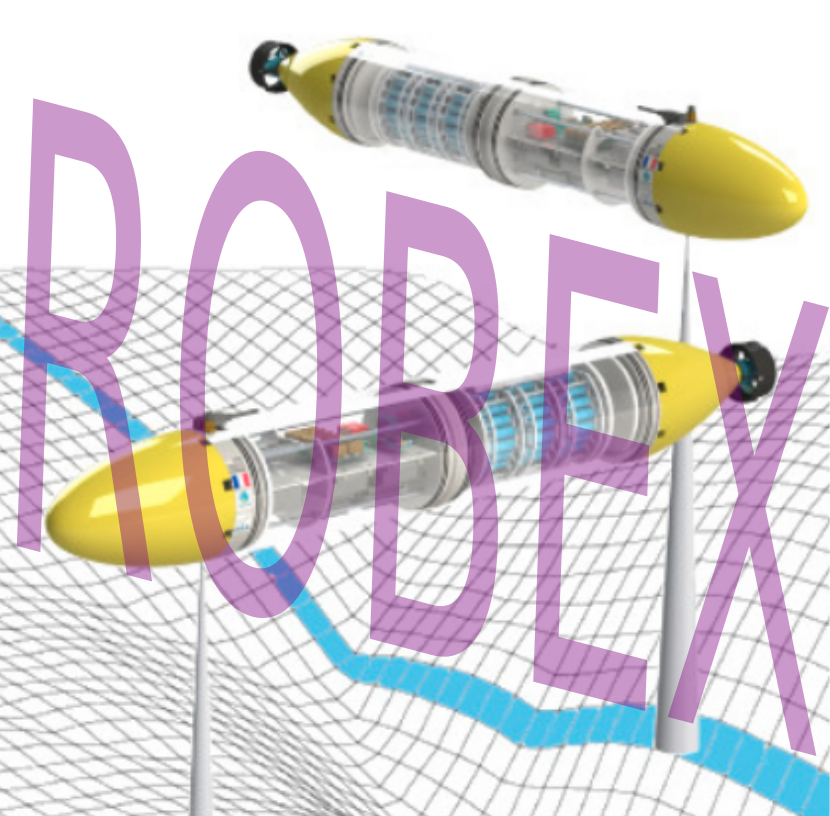
\includegraphics[height=0.75cm]{imgs/logo_robex}}
    \end{tabular}
}

\begin{document}

    \maketitle

    \section{Introduction}

        \begin{frame}{Motivations}
            \begin{block}<+->{Necessity of low-cost marine robots}
                \begin{itemize}
                    \item Marine robotics is a growing field with applications in environmental monitoring, underwater exploration, and resource management.
                    \item Low-cost solutions are essential for widespread adoption, and swarm experimentation in marine robotics.
                \end{itemize}
            \end{block}
        \end{frame}

        \begin{frame}{Existing Solutions}
            \begin{figure}
                \centering
                \begin{subfigure}[c]{0.4\textwidth}
                    \centering
                    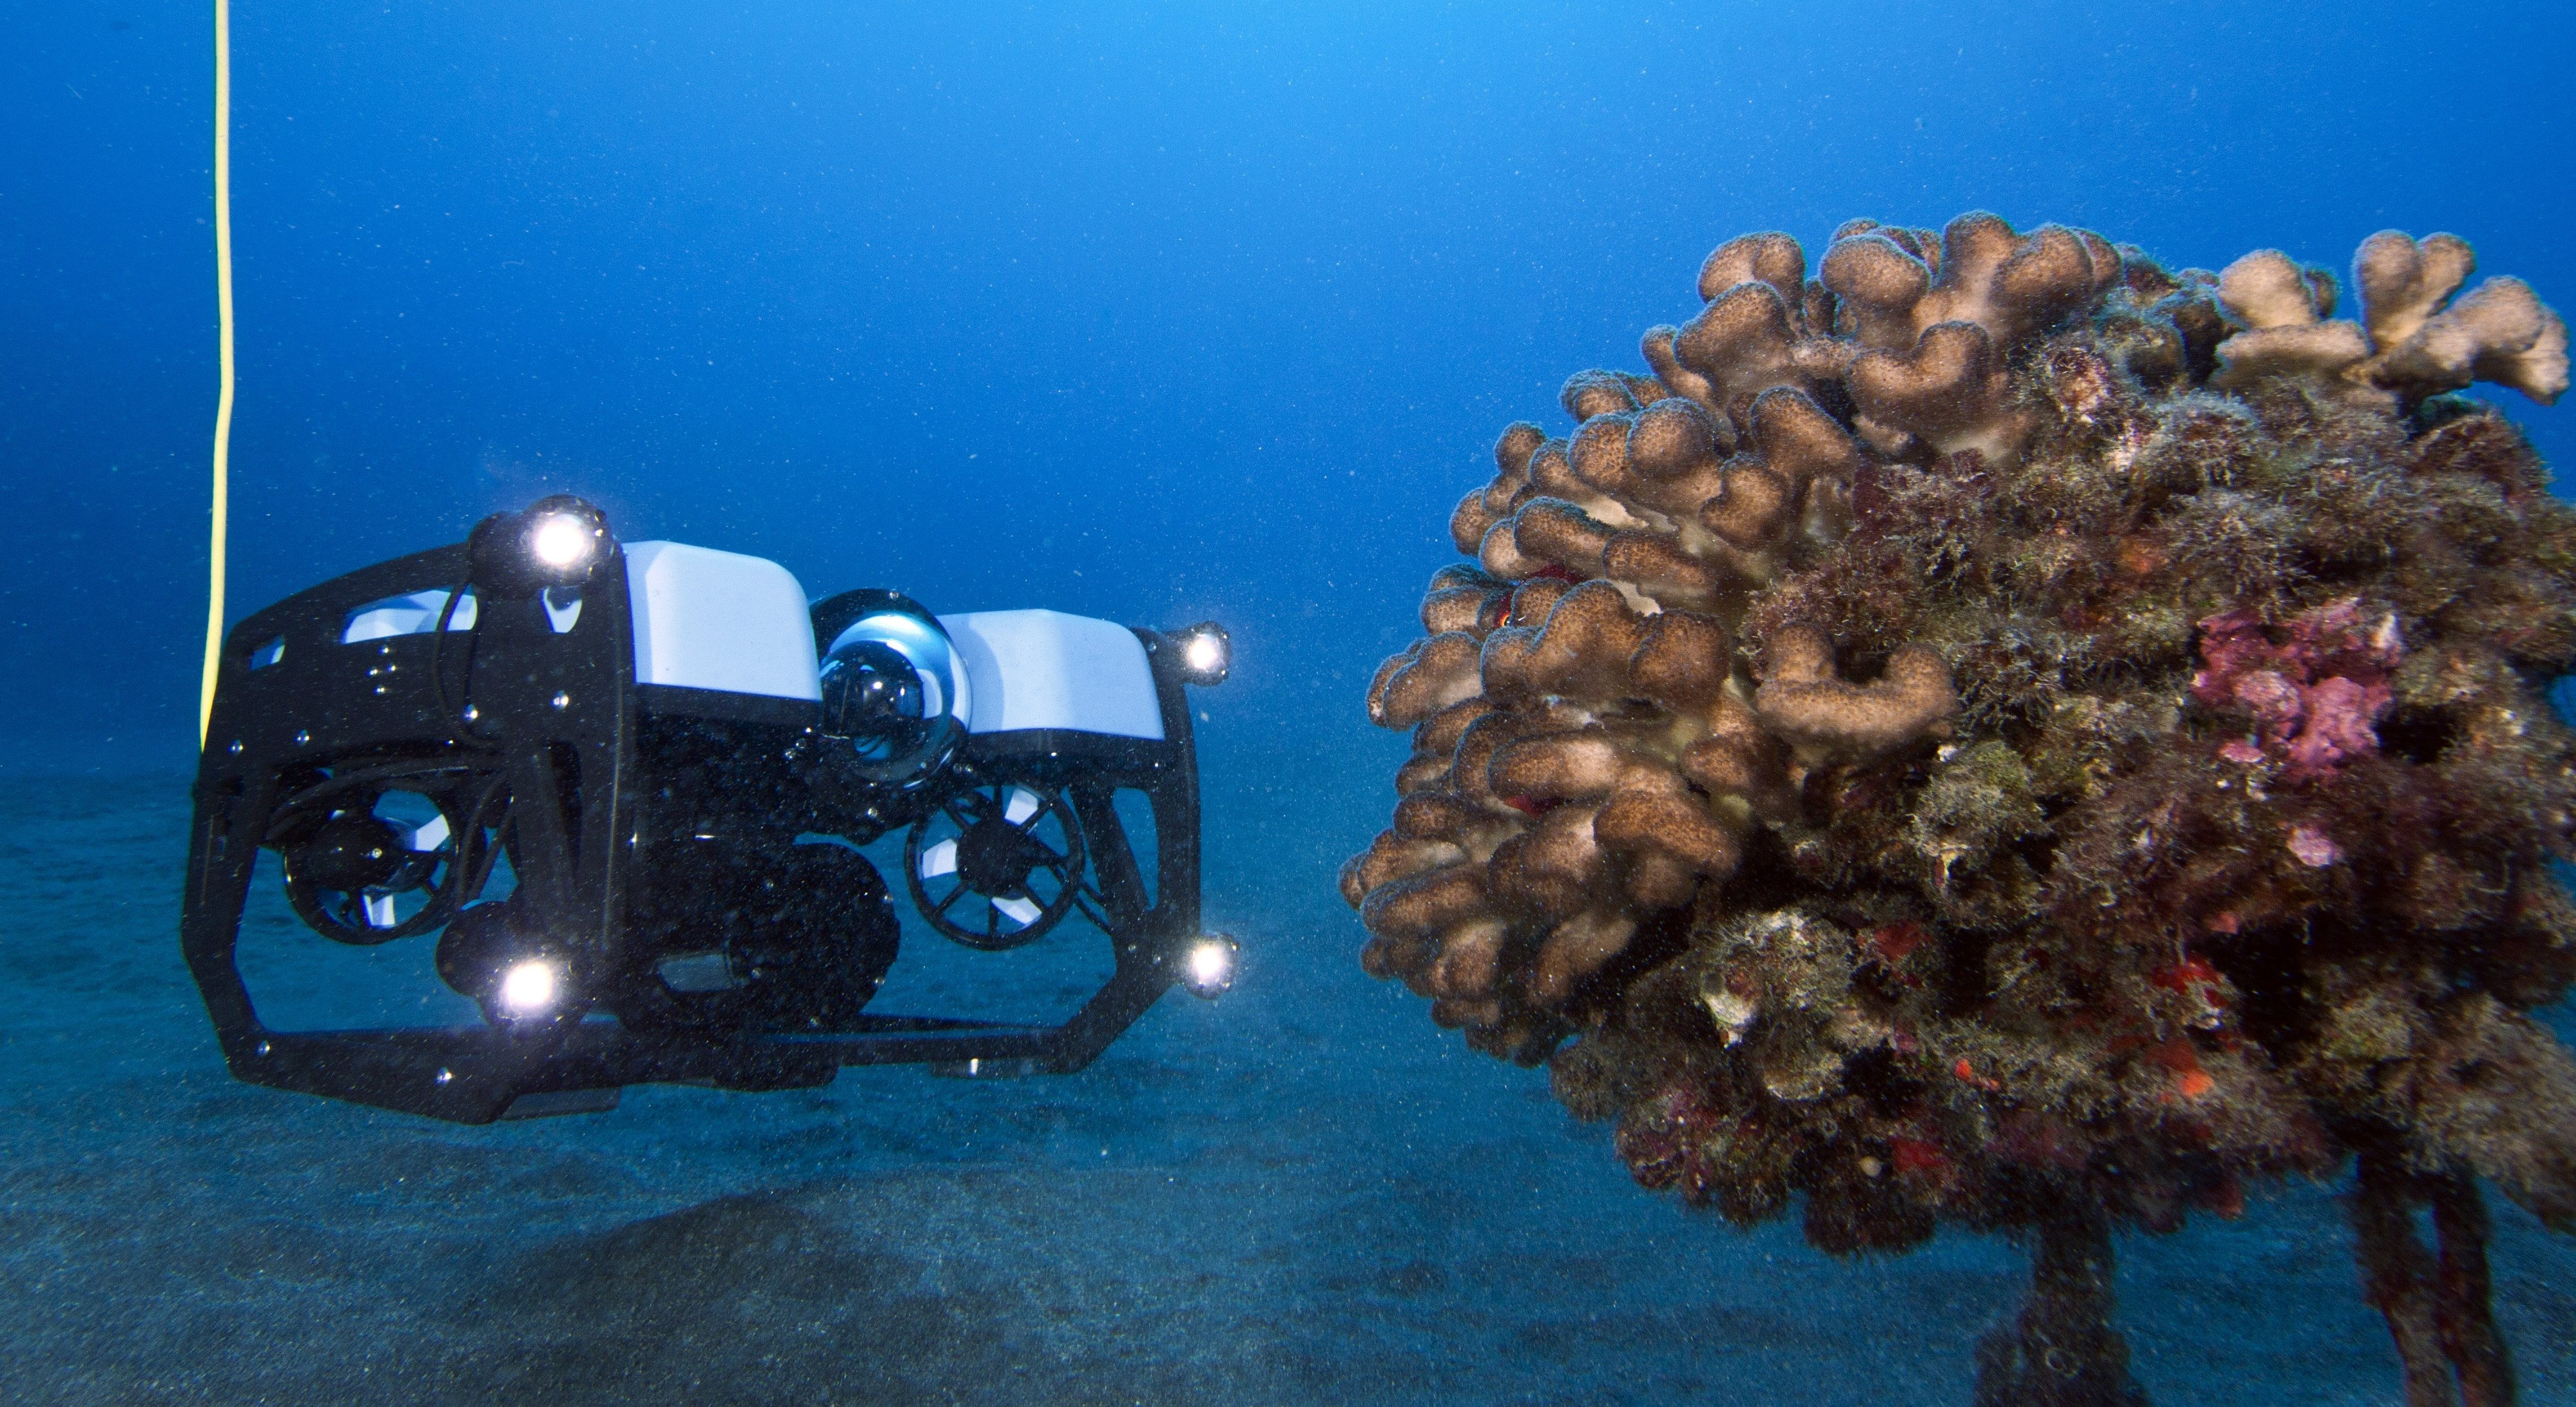
\includegraphics[width=\textwidth]{imgs/bluerov2.jpg}
                    \caption{BlueROV2 (Blue Robotics)}
                \end{subfigure}
                \begin{subfigure}[c]{0.4\textwidth}
                    \centering
                    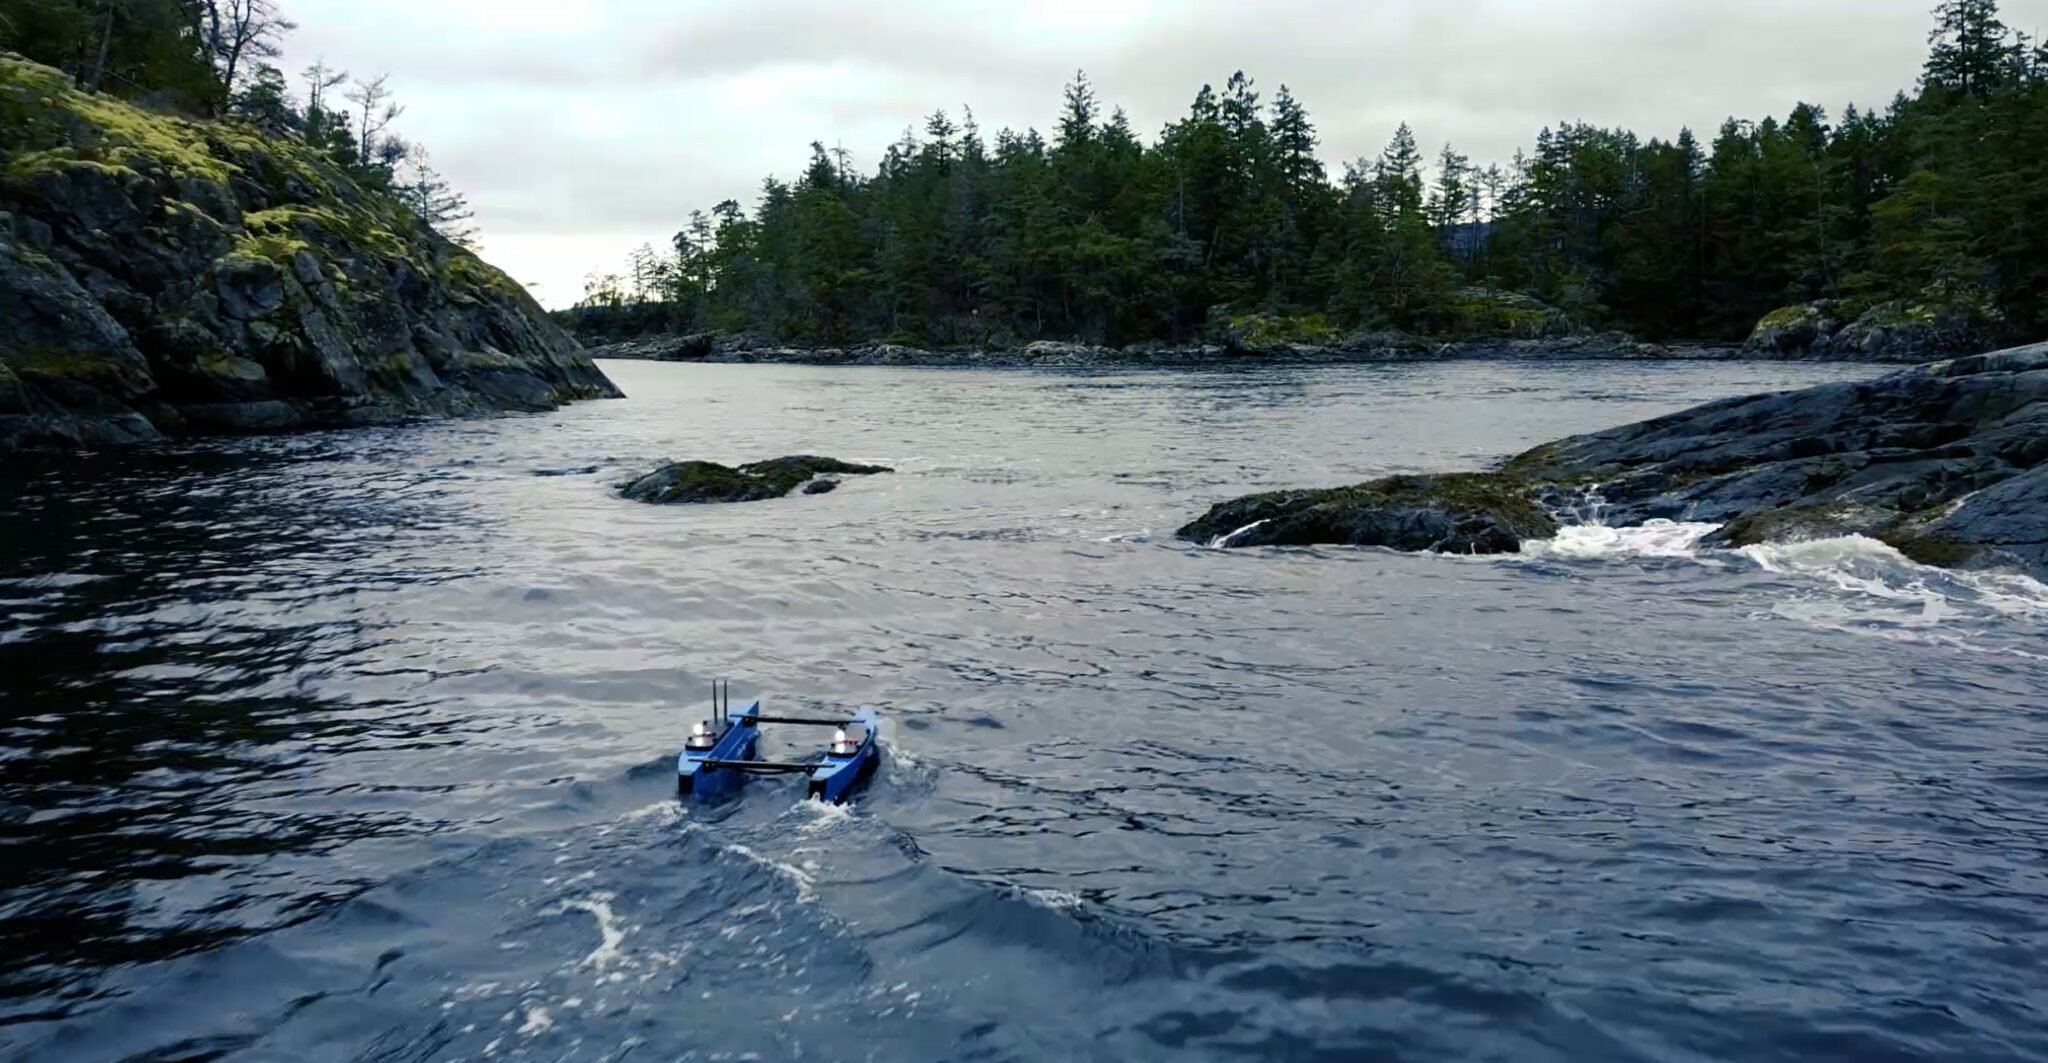
\includegraphics[width=\textwidth]{imgs/blueboat.jpg}
                    \caption{BlueBoat (Blue Robotics)}
                \end{subfigure}
                \begin{subfigure}[c]{0.4\textwidth}
                    \centering
                    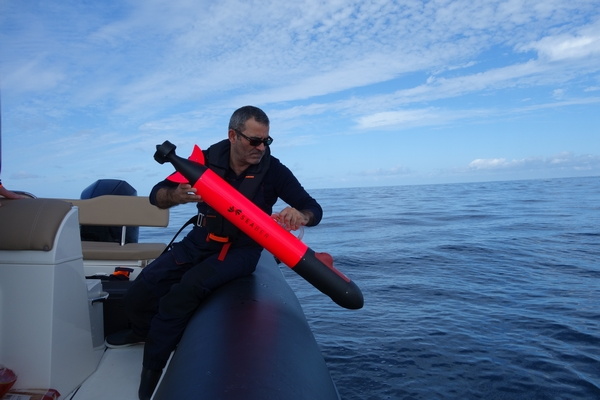
\includegraphics[width=\textwidth]{imgs/yuco.jpg}
                    \caption{Yuco (Seaber)}
                \end{subfigure}
                \begin{subfigure}[c]{0.4\textwidth}
                    \centering
                    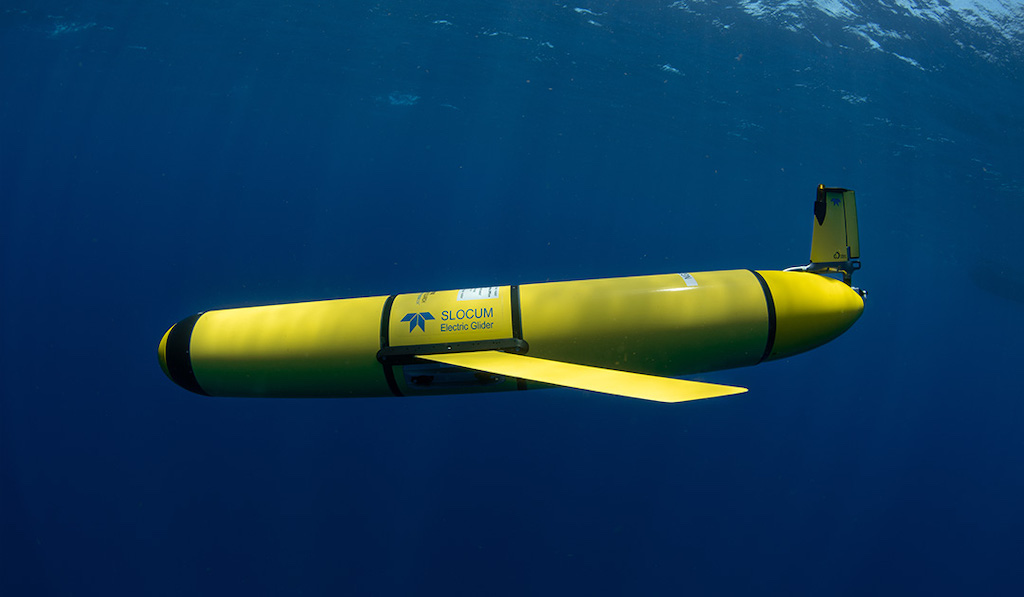
\includegraphics[width=\textwidth]{imgs/slocum.jpg}
                    \caption{Slocum (Teledyne Webb Research)}
                \end{subfigure}
                \caption{Small marine robots}
            \end{figure}
        \end{frame}

        \begin{frame}{Objectives}
            \begin{block}<+->{Main Objective}
                \begin{itemize}
                    \item Design a subsurface robot low-cost / low-tech
                    \item Use minimal number of actuators and sensors
                    \item Ensure ease of build and maintenance
                \end{itemize}
            \end{block}

            \begin{block}<+->{Benefits}
                \begin{itemize}
                    \item Low visual, radar, and acoustic signatures
                    \item Reduced drag and improved hydrodynamics
                    \item Enhanced stability and maneuverability
                \end{itemize}
            \end{block}
        \end{frame}

    \section{Modeling}
    
        \begin{frame}{Longitudinal Stability of Aerial Vehicles}
            \begin{figure}
                \centering
                \begin{overprint}
                    \only<1>{
                        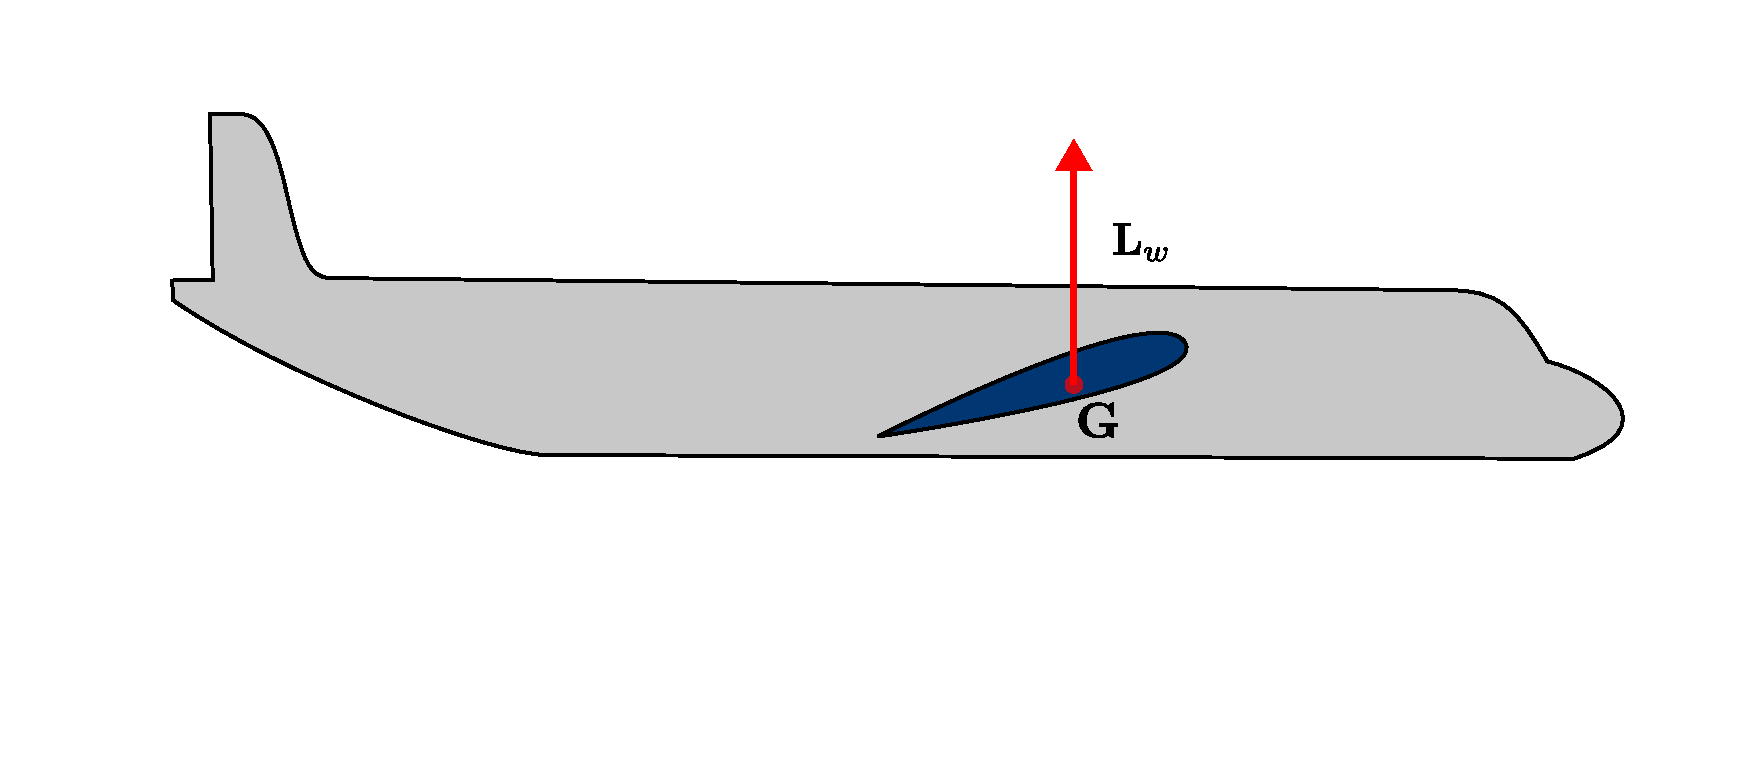
\includegraphics[width=\textwidth]{imgs/plane_1wing}
                        \caption{1 wing plane}
                    }
                    \only<2>{
                        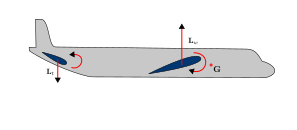
\includegraphics[width=\textwidth]{imgs/plane_2wings}
                        \caption{2 wing plane}
                    }
                \end{overprint}
            \end{figure}
        \end{frame}

        \begin{frame}{Longitudinal Stability of the Subsurface}
            \begin{figure}
                \centering
                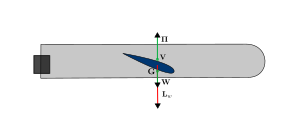
\includegraphics[width=\textwidth]{imgs/subsurface_1wing}
                \caption{1 wing subsurface}
            \end{figure}
        \end{frame}

        \begin{frame}{Physical Model}
            \begin{block}{Forces}
                \begin{itemize}
                    \item Weight $\mathbf{W} = m \mathbf{g}$
                    \item Buoyancy $\boldsymbol{\Pi} = -\rho V \mathbf{g}$
                    \item Thrust $\mathbf{F}_x$ from the thruster
                    \item Body Drag $\mathbf{D}_b = \frac{1}{2} \rho C_{D, b} A \mathbf{}u |\mathbf{}u|$
                    \item Wings Lift $\mathbf{L} = \frac{1}{2} \rho C_L S \mathbf{}u |\mathbf{}u|$
                    \item Wings Drag $\mathbf{D} = \frac{1}{2} \rho C_D S \mathbf{}u |\mathbf{}u|$
                \end{itemize}
            \end{block}
            \begin{block}<+->{Equations of motion}
                \begin{equation}
                    \left\{
                    \begin{aligned}
                        m \ddot x &= F_x - \frac{1}{2} \rho (C_{D, b} A + C_D S) \dot x |\dot x| \\
                        m \ddot z &= (m - \rho V) g + \frac{1}{2} \rho C_L S \dot x |\dot x|
                    \end{aligned}
                    \right.
                \end{equation}
            \end{block}
        \end{frame}

        \begin{frame}{Equilibrium Computation}
            \begin{block}<+->{Cruise Speed}
                \begin{equation}
                    \dot x^* = \sqrt{\frac{2 F_x}{\rho (C_{D, b} A + C_D S)}}
                \end{equation}
            \end{block}
            \begin{block}<+->{Equilibrium Vertical Acceleration}
                \begin{equation}
                    F_x = \frac{\rho (C_{D, b} A + C_D S)}{2} \sqrt{\frac{2 (\rho V - m) g}{\rho C_L S}}
                \end{equation}
            \end{block}
        \end{frame}

    \section{Robot Design}

        \begin{frame}{Design Considerations}
            \begin{block}<+->{Material Selection}
                \begin{itemize}
                    \item PMMA tube for the main body
                    \item 3D-printed parts (FDM / SLA)
                    \item Simple microcontroller (ESP32 / Arduino)
                \end{itemize}
            \end{block}
            \begin{block}<+->{Actuators and Sensors}
                \begin{itemize}
                    \item Two thrusters for propulsion and steering
                    \item Pressure sensor for depth measurement
                    \item Basic Accelerometer / Gyroscope / Magnetometer (IMU)
                    \item GNSS receiver for surface positioning
                \end{itemize}
            \end{block}
        \end{frame}

        \begin{frame}{CAD Model}
            \begin{figure}
                \centering
                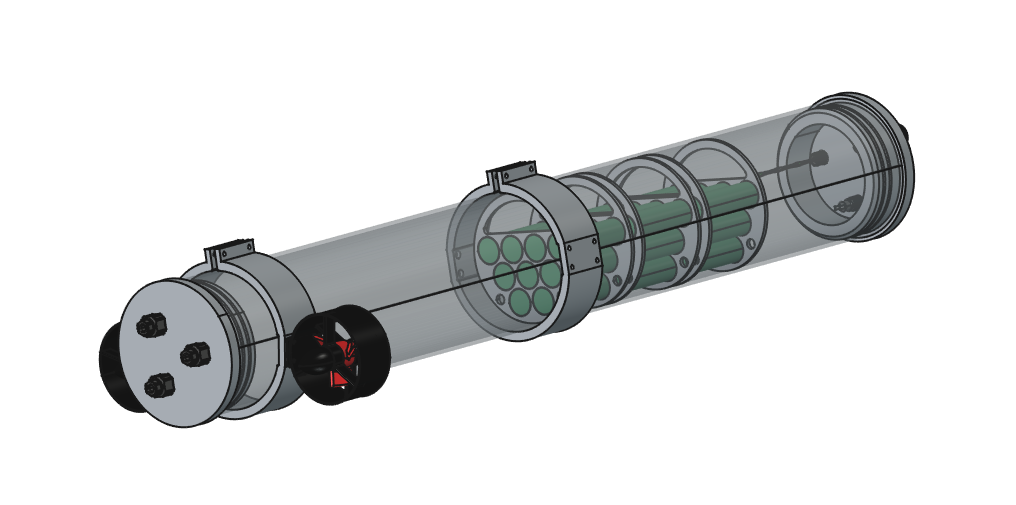
\includegraphics[width=0.8\textwidth]{imgs/cad.png}
                \caption{CAD model of the subsurface robot}
            \end{figure}
        \end{frame}

        \begin{frame}{Subsurface Robot Prototype}
            \begin{figure}
                \centering
                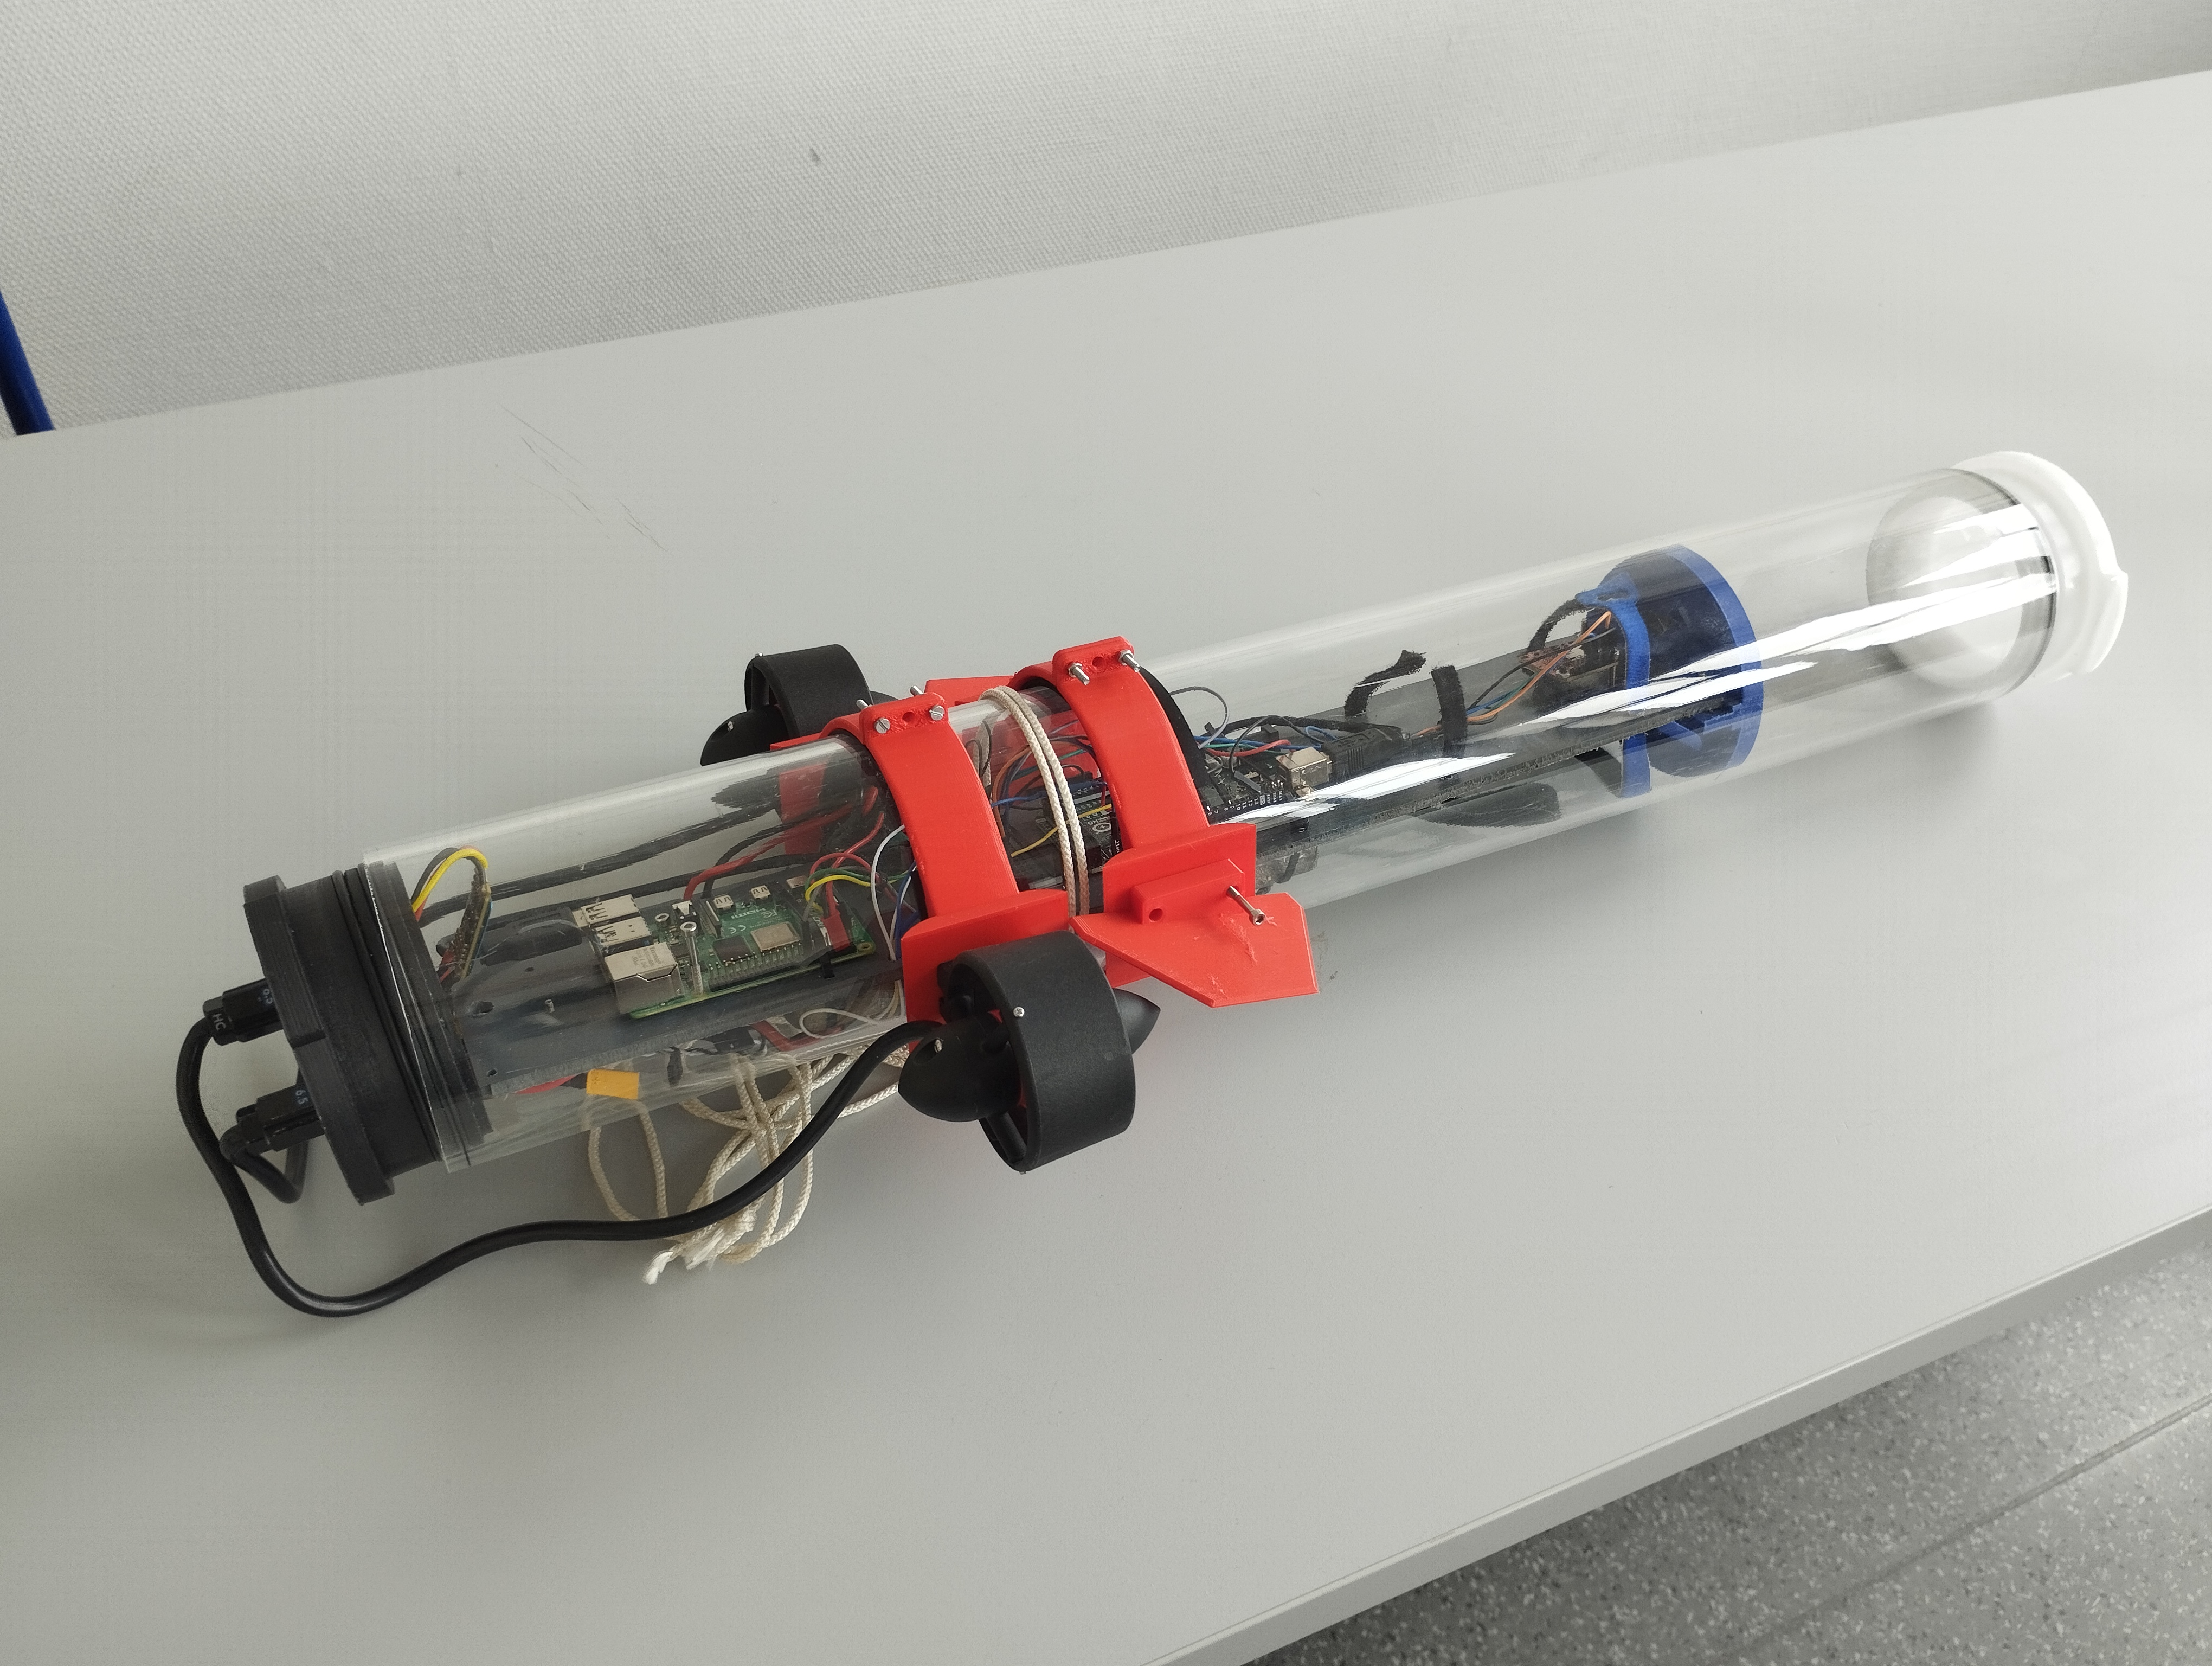
\includegraphics[width=0.8\textwidth]{imgs/subsurface.jpg}
                \caption{Subsurface robot prototype}
            \end{figure}
        \end{frame}

    \section{Depth Controller}

        \begin{frame}{Depth Control Strategies}
            \begin{figure}
                \resizebox{\textwidth}{!}{
                    \begin{tikzpicture}[box/.style={font=\sffamily, rectangle, minimum height=1cm, minimum width=1cm, fill=ENSTABlue!15, draw=ENSTABlue}, node distance=1cm, auto]
                        \node (u) {};
                        \node[box, right=1cm of u] (thruster) {Thruster};
                        \node[box, right=1cm of thruster] (int1) {$\int$};
                        \node[box, right=1cm of int1] (lift) {Wings};
                        \node[box, right=1cm of lift] (int2) {$\int$};
                        \node[box, right=1cm of int2] (int3) {$\int$};
                        \node[right=1cm of int3] (depth) {};

                        \draw[->, >=latex] (u) -- node[midway, above] {$u$} (thruster);
                        \draw[->, >=latex] (thruster) -- node[midway, above] {$\mathbf{F}_x$} (int1);
                        \draw[->, >=latex] (int1) -- node[midway, above] {$\dot{x}$} (lift);
                        \draw[->, >=latex] (lift) -- node[midway, above] {$\mathbf{F}_z$} (int2);
                        \draw[->, >=latex] (int2) -- node[midway, above] {$\dot{z}$} (int3);
                        \draw[->, >=latex] (int3) -- node[midway, above] {$z$} (depth);
                    \end{tikzpicture}
                }
                \caption{Diagram of the Input / Output relationship for depth control}
            \end{figure}
        \end{frame}

        \begin{frame}{Sliding Mode Control}
            \begin{block}<+->{Dynamical system}
                \begin{equation}
                    \dot{\mathbf{x}} = f(\mathbf{x},t) + g(\mathbf{x},t)\mathbf{u}
                \end{equation}
            \end{block}
            \begin{block}<+->{Sliding Surface}
                \begin{equation}
                    \boldsymbol{\sigma}(\mathbf{x},t) = \left(\frac{d}{dt} + \lambda\right)^{(n-1)} (\mathbf{x} - \mathbf{x}_d)
                \end{equation}
            \end{block}
            \begin{block}<+->{Sliding Mode Controller}
                Ensures $\boldsymbol{\sigma}(\mathbf{x},t)\to 0$
                \begin{equation}
                    \mathbf{u} = \mathbf{u}_{\text{eq}} - k \,\mathrm{sign}(\boldsymbol{\sigma})
                \end{equation}
            \end{block}
        \end{frame}

        \begin{frame}{SMC for Depth Control}
            \begin{block}<+->{Sliding Surface}
                \begin{equation}
                    \sigma(\mathbf{x}, t) = (\dot z - \dot z_d) + (z - z_d)
                \end{equation}
            \end{block}
            \begin{block}<+->{Finite-time convergence}
                \begin{equation}
                    F_x = - sign(\sigma(\mathbf{x}, t))
                \end{equation}
            \end{block}
            \begin{block}<+->{Asymptotic convergence}
                \begin{equation}
                    F_x = - tanh(\sigma(\mathbf{x}, t))
                \end{equation}
            \end{block}
        \end{frame}

        \begin{frame}{Simulation Results}
            \begin{figure}
                \begin{subfigure}{.5\textwidth}
                    \centering
                    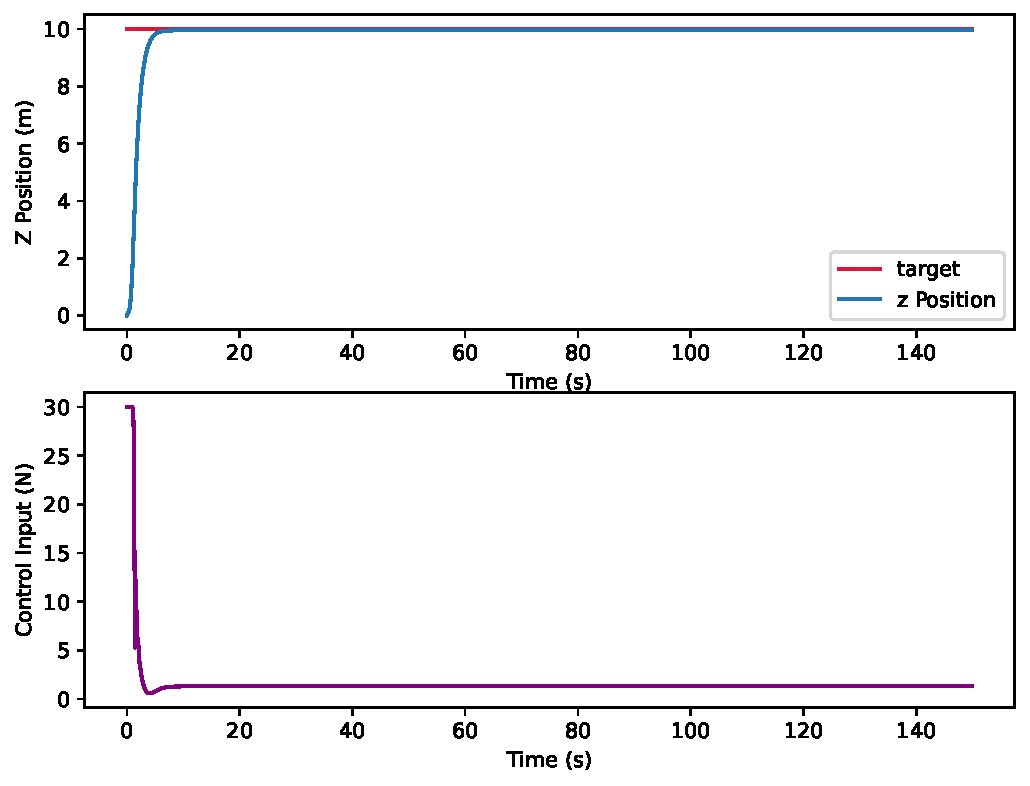
\includegraphics[width=\textwidth]{imgs/smc_control_setpoint.pdf}
                    \caption{Setpoint}
                \end{subfigure}%
                \begin{subfigure}{.5\textwidth}
                    \centering
                    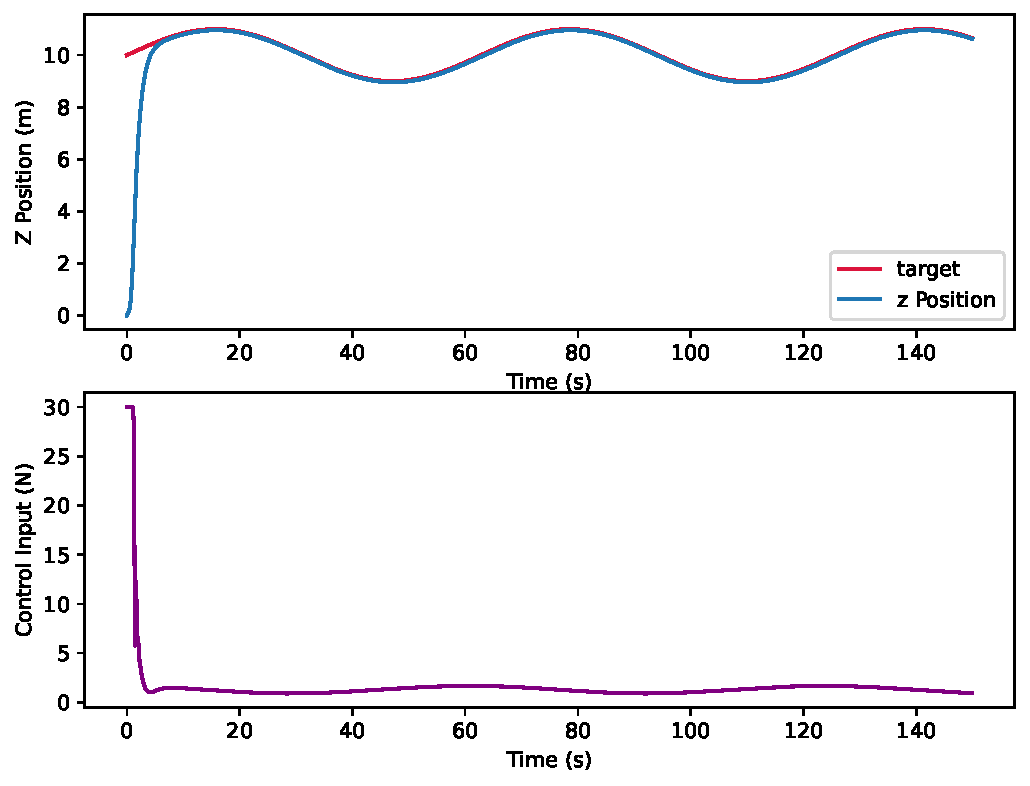
\includegraphics[width=\textwidth]{imgs/smc_control_tracking.pdf}
                    \caption{Tracking}
                \end{subfigure}
                \caption{Simulation results of SMC depth control}
            \end{figure}
        \end{frame}

    \section{Conclusion}

        \begin{frame}{Conclusion and Future Work}
            \begin{block}<+->{Conclusion}
                \begin{itemize}
                    \item Successfully designed a low-cost subsurface robot model
                    \item Developed a sliding mode control strategy for depth regulation
                    \item Simulation results demonstrate effective depth tracking
                \end{itemize}
            \end{block}
            \begin{block}<+->{Future Work}
                \begin{itemize}
                    \item Build and test the physical robot in real-world conditions
                    \item Implement and validate the control algorithm on hardware
                    \item Test fast navigation strategies
                \end{itemize}
            \end{block}
        \end{frame}

    \maketitle

    % Backup slides
    % \appendix

\end{document}